\section{Conformal field theory}\label{ss:CFT}

In this section, we consider QFTs invariant under the conformal transformation
\begin{align}\label{ConfTra}
\bar g_{\mu\nu}(x') = \Omega^2 (x)\, g_{\mu\nu}(x) \ ,
\end{align}
where $\bar g_{\mu\nu}$ is the transformed metric.
In Euclidean space $\BR^{d}$, the group of the conformal transformation is $\SO (1,d+1)$ while in Minkowski space $\BR^{1,d-1}$ the group is $\SO (2,d)$.
The conformal group is an extension of the Poincar{\'e} group, including the dilatation $x'^\mu = \lambda\, x^\mu$ for a constant $\lambda$ and the special conformal transformation $x'^\mu = (x^\mu + b^\mu x^2)/(1+ 2b_\mu x^\mu + b^2 x^2)$ for a vector $b^\mu$, hence preserving the angle between two curves infinitesimally \cite{DiFrancesco:1997nk}.


Let $I_E[g_{\mu\nu}, \phi ]$ be the Euclidean action for a theory with a field $\phi(x)$ and a metric $g_{\mu\nu}$.
This theory is called classical conformal field theory if the action does not change under the following transformation:
\begin{align}
	I_E[\bar g_{\mu\nu}, \bar \phi ] =  I_E[ g_{\mu\nu}, \phi ] \ ,\qquad \bar \phi(x') = \Omega^{-\Delta} (x)\, \phi(x) \ ,
\end{align}
for some constant $\Delta$ being the conformal dimension of the field $\phi(x)$.
For example, a scalar field theory coupled to a curved space 
\begin{align}\label{ConfScalar}
	I_E[g_{\mu\nu}, \phi ] = \frac{1}{2} \int \d^d x \sqrt{g}\, \left[ \partial_\mu\phi\, \partial^\mu \phi + \frac{d-2}{4(d-1)} \CR\, \phi^2 \right] 
\end{align}
is conformally invariant with $\Delta = d/2 -1$.
It is straightforward to check that Eq.\,\eqref{ConfScalar} is conformal invariant  using the transformation law of the Ricci scalar \cite{Birrell:1982ix}:
\begin{align}\label{RicciConfTr}
\begin{aligned}
	\CR [\bar g_{\mu\nu}] &= \Omega^{-2} \CR[g_{\mu\nu}] - 2(d-1)\Omega^{-3}\,\nabla^2\Omega \\
		&\qquad - (d-1)(d-4)\Omega^{-4} \partial_\mu\Omega\, \partial^\mu\Omega \ ,
\end{aligned}
\end{align}
where the covariant derivatives on the right-hand side are taken with respect to the metric $g_{\mu\nu}$ before the conformal transformation.
An equivalent, but a slightly simpler way to derive Eq.\,\eqref{ConfScalar} is to construct a conformal invariant $\phi^{d/\Delta} \sqrt{g} \,\CR[\phi^{2/\Delta}g_{\mu\nu}]$ out of the metric and the scalar field and use Eq.\,\eqref{RicciConfTr} with $\Omega = \phi^{1/\Delta}$.
To make it quadratic in $\phi$, one needs to set $\Delta = d/2 - 1$ for the conformal dimension \cite{Brown:1976wc} and finds
\begin{align}
\begin{aligned}
	\phi^{d/\Delta} \,\CR[\phi^{2/\Delta}g_{\mu\nu}] &= \phi^2\, \CR[g_{\mu\nu}] \\
		&\qquad + \frac{4(d-1)}{d-2}\left[ \partial_\mu \phi \partial^\mu\phi - \nabla^\mu (\phi \partial_\mu \phi)\right] \ .
\end{aligned}
\end{align}
This gives the conformal invariant action \eqref{ConfScalar} up to the total derivative and normalization.

Next, consider an action $I_E[g_{\mu\nu}]$ of the metric, which may be obtained by integrating out all fields on a curved space. 
The variation of the action under the infinitesimal conformal transformation $\delta g_{\mu\nu} = 2\,\delta \Omega (x) g_{\mu\nu}$ becomes
\begin{align}
\delta I_E[g_{\mu\nu}] = \int \d^d x\,\delta g_{\mu\nu} \frac{\delta I_E[g_{\mu\nu}]}{\delta g_{\mu\nu}} =\int \d^d x \sqrt{g}\, T_{\mu}^{~\mu}\, \delta \Omega(x) \ ,
\end{align}
where the stress-energy tensor is defined by
\begin{align}\label{STDef}
T^{\mu\nu} = \frac{2}{\sqrt{g}} \frac{\delta I_E}{\delta g_{\mu\nu}} \ .
\end{align}
If the theory is conformally invariant, the action has to be invariant under any deformation $\delta \Omega(x)$; hence the trace of the stress-energy tensor has to vanish, $T_\mu^{~\mu} = 0$.

The traceless property of the stress tensor at the classical level is violated at the quantum mechanical level due to the conformal anomaly in even dimensions \cite{Bonora:1985cq,Duff:1993wm,Deser:1993yx}, which can be put in the form
\begin{align}\label{WeylAnomaly}
\langle T_\mu^{~\mu} \rangle = \frac{(-1)^{d/2}}{2} A\, E_{d} - \sum_i B_i \,I_i + \nabla_\mu J^\mu\ ,
\end{align}
where $E_{d}$ is the Euler density, normalized so that $\int_{\BS^{d}} E_{d} = 2$, and $I_i$ are a set of the independent Weyl invariants built from the Weyl tensor in $d$ dimensions.
The coefficients $A$ and $B_i$ are referred to as type $A$ and $B$ central charges, respectively.
The total derivative term $\nabla_\mu J^\mu$ is scheme dependent as it can be affected by adding local counterterms to the effective action.\footnote{For example, there is a total derivative term $\nabla_\mu J^\mu \propto \Box\, \CR$ in four dimensions, which can be removed by a local counterterm $\CR^2$ \cite{Birrell:1982ix}.}
Thus we ignore the total derivative term contribution to the conformal anomaly in the following discussion.


\subsection{Correlation functions}
The conformal symmetry restricts the form of correlation functions more severely than the Poincar{\'e} symmetry.
We start with a primary scalar operator $\CO(x)$ of conformal dimension $\Delta$  transforming under the conformal transformation Eq.\,\eqref{ConfTra} as
\begin{align}\label{ScaleTr}
	\bar \CO (x') = \Omega^{-\Delta}(x)\, \CO(x) \ .
\end{align}
The translation invariance imposes the constancy of the one-point function $\langle \CO(x)\rangle = c$, but the scaling law \eqref{ScaleTr} implies $c = \Omega^{-\Delta}(x)\, c$ for any $\Omega(x)$, thus the one-point function vanishes:
\begin{align}
	\langle \CO(x)\rangle = 0 \ .
\end{align}


Similarly the two-point function $\langle \CO_1(x)\,\CO_2(y)\rangle$ of primary operators $\CO_1$ and $\CO_2$ of conformal dimensions $\Delta_1$ and $\Delta_2$ depends only on the distance $|x-y|$ between the two points by the translation invariance. 
To incorporate the dilatation and the special conformal invariances, the two conformal dimensions should be the same. 
Then the two-point function of appropriately normalized operators takes the form
\begin{align}\label{TwoPnt}
	\langle \CO_1(x)\,\CO_2(y)\rangle = \frac{\delta_{\Delta_1\, \Delta_2}}{|x-y|^{2\Delta_1}}  \ .
\end{align}

The three-point function of primary operators $\CO_1, \CO_2$ and $\CO_3$ of conformal dimensions $\Delta_1, \Delta_2$ and $\Delta_3$ are similarly fixed by the conformal symmetry,
\begin{align}
\begin{aligned}
	\langle &\CO_1(x)\,\CO_2(y) \, \CO_3(z)\rangle \\
	&= \frac{C_{123}}{|x-y|^{\Delta_1 + \Delta_2 - \Delta_3}|y-z|^{\Delta_2 + \Delta_3 - \Delta_1}|z-x|^{\Delta_3 + \Delta_1 - \Delta_2}} \ ,
\end{aligned}
\end{align}
where $C_{123}$ is an undetermined constant.
Correlation functions of more than four operators cannot be completely fixed by only the conformal invariance in this way. 


For conserved currents $j_\mu(x)$ of dimension $\Delta=d-1$ and the stress tensor $T_{\mu\nu}(x)$ of dimension $d$, their one-point functions vanish and the two-point functions are fixed to be \cite{Osborn:1993cr,Erdmenger:1996yc}
\begin{align}\label{jjCor}
	\langle j_\mu(x)\, j_\nu(y) \rangle = C_J\, \frac{I_{\mu\nu}(x-y)}{(x-y)^{2(d-1)}} \ ,
\end{align}
and
\begin{align}\label{TTCor}
\langle T_{\mu\nu}(x)\,T_{\rho\sigma}(y)\rangle
	= C_T\, \frac{I_{\mu\nu,\rho\sigma}(x-y)}{(x-y)^{2d}} \ ,
\end{align}
with the conformally invariant functions,
\begin{align}
\begin{aligned}
I_{\mu\nu}(x) &= \delta_{\mu\nu} - \frac{2x_\mu x_\nu}{x^2} \ , \\
I_{\mu\nu,\rho\sigma}(x) &= \frac{1}{2}\left[ I_{\mu\rho}(x)I_{\nu\sigma}(x) +I_{\mu\sigma}(x)I_{\nu\rho}(x) \right] -\frac{1}{d}\delta_{\mu\nu}\delta_{\rho\sigma} \ .
\end{aligned}
\end{align}
The two-point functions of a scalar primary field $\CO(x)$ and the conserved current or the stress tensor vanish,
\begin{align}\label{TO_CFT}
	\langle j(x)\, \CO(y)\rangle = \langle T_{\mu\nu} (x)\, \CO(y) \rangle = 0 \ ,
\end{align}
due to the conformal invariance and the conservation laws $\partial_\mu j^\mu = 0$ and $\partial_\mu T^{\mu\nu} = 0$.



\subsection{Conformal anomaly in entanglement entropy}
We saw in the previous section that entanglement entropy has the UV divergences whose leading part is always proportional to the area of the entangling surface $\Sigma$ in Eq.\,\eqref{EAfinite}.
There are also universal logarithmic divergences depending on whether $d$ is even or not.
We show this logarithmic divergence is induced by the conformal anomaly Eq.\,\eqref{WeylAnomaly} of the stress-energy tensor in even $d$ dimensions.

Let us consider the scale transformation of the entanglement entropy of an entangling surface $\Sigma$ of size $l$.
We need to know how the partition function $Z_n$ on the $n$-fold cover $\CM_n$ transforms under the Weyl scaling $l \to e^{\sigma} l$.
Equivalently we act the scaling of the metric $g_{\mu\nu} \to e^{2\sigma}g_{\mu\nu}$ on the effective action $\log Z_n$ and read off the variation locally given by the expectation value of the stress tensor on $\CM_n$:
\begin{align}
l \frac{\d}{\d l}\, \log Z_n = -\int_{\CM_n} \d^d x \sqrt{g}\, \langle T_\mu^{~\mu} \rangle \ .
\end{align} 
It follows with the QFT definition Eq.\,\eqref{EE_PF} that the entanglement entropy varies under the scale transformation as
\begin{align}\label{EE_Weyl}
l \frac{\d}{\d l}\, S_A = -\int_{\CM_1} \d^d x \sqrt{g}\, \langle T_\mu^{~\mu} \rangle + \lim_{n\to 1} \partial_n \int_{\CM_n} \d^d x \sqrt{g}\, \langle T_\mu^{~\mu} \rangle \ .
\end{align}
In odd dimensions, $\langle T_\mu^{~\mu} \rangle = 0$ for CFTs and there are no logarithmic divergences in the entropy.
On the other hand, the right hand side can be nonvanishing due to the conformal anomaly, Eq.\,\eqref{WeylAnomaly}, in even dimensions.
If a theory is defined on a flat space ($\CM_1 = \BR^d$), the first term always vanishes while the second term has a nontrivial contribution from the conical singularity at the entangling surface $\Sigma$.
In what follows, we estimate the second term explicitly using Eqs.\,\eqref{SingularFormulae1}-\eqref{SingularFormulae4} in two and four dimensions.

In two dimensions, the Euler density is $E_2 = \CR/(4\pi)$ while there are no Weyl invariants.
We rescale the type $A$ central charge, $A = c/3$, so as to follow the canonical convention in CFT$_2$.
Then substituting the trace of the stress tensor
\begin{align}
\langle T_\mu^{~\mu} \rangle = - \frac{c}{24\pi}\CR \ ,
\end{align}
into Eq.\,\eqref{EE_Weyl} and applying Eq.\,\eqref{SingularFormulae1}, we find the entanglement entropy for an interval of width $l$,
\begin{align}
l \frac{\d}{\d l}\, S_A = \frac{c}{6}\int_\Sigma 1 = \frac{c}{3} \ .
\end{align}
This result yields a well-known behavior of entanglement entropy of CFT$_2$ \cite{Holzhey:1994we,jin2004quantum,Calabrese:2004eu}
\begin{align}\label{EE_CFT2}
S_A = \frac{c}{3}\log \frac{l}{\epsilon} + \cdots \ ,
\end{align}
where $\epsilon$ is a UV cutoff and $\cdots$ are finite parts.

In four dimensions, there is one Euler density and one Weyl invariant,
\begin{align}
\begin{aligned}
E_4 &= \frac{1}{32\pi^2} \left( \CR_{\mu\nu\rho\sigma}^2 - 4 \CR_{\mu\nu}^2 + \CR^2 \right) \ , \\
I_4 &= \frac{1}{16\pi^2} \left( \CR_{\mu\nu\rho\sigma}^2 - 2 \CR_{\mu\nu}^2 + \frac{1}{3}\CR^2 \right) \ ,
\end{aligned}
\end{align}
whose coefficients we conventionally take to be $A = a$ and $B=c$, respectively.
Again, Eqs.\,\eqref{SingularFormulae1}-\eqref{SingularFormulae4} and the identities \eqref{WeylAnomaly} and \eqref{EE_Weyl} lead to the logarithmic divergence of entanglement entropy in CFT$_4$:
\begin{align}\label{EE_4d}
S_A = \frac{c_2}{\epsilon^2} + c_0\log \frac{l}{\epsilon}  + \cdots \ ,
\end{align}
where $c_2$ is a constant proportional to the area $A_\Sigma$ of the entangling surface $\Sigma$ and $c_0$ is fixed to be \cite{Solodukhin:2008dh,Fursaev:2013fta}
\begin{align}\label{c04d}
\begin{aligned}
c_0 &=-\frac{a}{2}\, \chi [\Sigma ]\\
	&\quad  + \frac{c}{2\pi} \int_\Sigma \left[ \CR_{abab} - \CR_{aa} + \frac{1}{3}\CR \right.\\
		&\qquad\qquad\qquad \left. + \frac{1}{2} (\CK^{a\,\mu}_{\,\mu})^2 - \CK^a_{\mu\nu} \CK^{a\,\mu\nu}\right] \ .
\end{aligned}
\end{align}
Here we used the Gauss-Codazzi equation \eqref{GaussCodazzi} relating the Ricci curvature on $\Sigma$ to the intrinsic and extrinsic curvatures,
which gives the first term proportional to the topological invariant (the Euler characteristic)
\begin{align}
	\chi[\Sigma]= \int_\Sigma E_2 = \frac{1}{4\pi}\int_\Sigma \CR_\Sigma \ ,
\end{align}
of the entangling surface $\Sigma$.
If the entangling surface is spherical, $\Sigma = \BS^2$, only the $a$-anomaly contributes to Eq.\,\eqref{c04d}, while if it is cylindrical $\Sigma = \BS^1 \times \BR$, only the $c$-anomaly survives.
The same expression \eqref{c04d} for the coefficient $c_0$ can be obtained by a holographic calculation in higher derivative gravities \cite{Hung:2011xb}, where the logarithmic divergences arise from a particular class of anomalies for a submanifold of even dimensions in CFT, known as the Graham-Witten anomalies \cite{Graham:1999pm}.


In higher dimensions, there is one Euler density and several independent Weyl invariants.
Entanglement entropy in even $d$-dimensional CFT allows the structure,
\begin{align}\label{EE_Even}
S_A = \frac{c_{d-2}}{\epsilon^{d-2}} + \frac{c_{d-4}}{\epsilon^{d-4}} + \cdots + \frac{c_2}{\epsilon^2} +  c_0\log \frac{l}{\epsilon}  + \cdots \ ,
\end{align}
with the logarithmic coefficient given by
\begin{align}\label{Log_EE_C0}
	c_0 = \frac{(-1)^{d/2+1}}{2}\, A \, \chi [\Sigma] - \sum_i\, B_i\,\left( \partial_n \, \int_{\CM_n} I_i\right)\bigg|_{n\to 1} \ .
\end{align}
The finite terms represented by the last dots depend on the regularization scheme and do not have any physical meaning.
On the other hand, entanglement entropy in odd $d$-dimensional CFT has similar expansions without the logarithmic term,
\begin{align}\label{EE_Odd}
S_A = \frac{c_{d-2}}{\epsilon^{d-2}} + \frac{c_{d-4}}{\epsilon^{d-4}} + \cdots + \frac{c_1}{\epsilon}  + (-1)^{(d-1)/2}F \ .
\end{align}
The finite part $F$ is {\it scheme independent} and physical observable.
The sign factor $(-1)^{(d-1)/2}$ is introduced for $F$ being positive in $d$ dimensions \cite{Klebanov:2011gs}, but there are no proofs for the positivity except for topological field theory where $F$ is the topological entanglement entropy that can be shown to be nonnegative \cite{Kitaev:2005dm,Levin:2006zz}.
We investigate the role of the finite part of entanglement entropy in odd dimensions in later sections.


\subsubsection{One interval in CFT$_2$}
One can derive the entanglement entropy of one interval Eq.\,\eqref{EE_CFT2} in CFT$_2$ on a flat space $\BC$ using purely CFT techniques.
Suppose the interval is placed between $z = -l/2$ and $l/2$ in the complex $z$ plane $\BC$.
We first map the interval to a semi-infinite line from the origin to the infinity by the transformation 
\begin{align}
	\zeta\equiv \frac{z+l/2}{z-l/2} \ .
\end{align}
Then we make use of the conformal transformation from the complex plane to a cylinder,
\begin{align}\label{ConfMapCyl}
w\equiv \tau + \i\, \varphi = \frac{\ell}{2\pi} \log \zeta \ ,
\end{align}
where $\ell$ is the circumference of the cylinder $\varphi \sim \varphi + \ell$ as $\zeta$ is the complex coordinate of $\BC$.\footnote{Although the final result does not depend on $\ell$, we keep track of the $\ell$ dependence so as to make the argument as general as possible.}
For a later convenience, we excise two small holes of radius $\epsilon$ at $z=\pm l/2$ to regularize the UV divergence \cite{Ohmori:2014eia}.
Then the interval or equivalently the semi-infinite line is mapped to the line at $\varphi=0$ ranging from $\tau=- \ell\, \log (l/\epsilon)/(2\pi)$ to $\ell\, \log (l/\epsilon)/(2\pi)$ (see Fig.\,\ref{fig:CFT2EE}).

Now we want to construct the $n$-fold cover $\CM_n$ of $\BC$ by gluing $n$ copies of the complex plane along the interval.
This is easy to carry out in the $w$ coordinates by just gluing $n$ sheets of cylinder at $\varphi = k\ell$ $(k=0,1,\cdots, n)$, resulting in one cylinder of circumference $n\ell$ as in Fig.\,\ref{fig:CFT2EE}.
Then the partition function on $\CM_n$ is mapped to the cylinder partition function,
\begin{align}\label{CylinderPF}
	Z[\CM_n] = \langle 0| \,e^{- \beta H}\, |0 \rangle \ ,
\end{align}
where $\beta$ is the regularized length of the cylinder
\begin{align}
	\beta \equiv \frac{\ell}{\pi}\log \frac{l}{\epsilon} \ ,
\end{align}
and $H$ is the Hamiltonian along $\tau$ that will be fixed.

			
\begin{figure}[h]
\centering
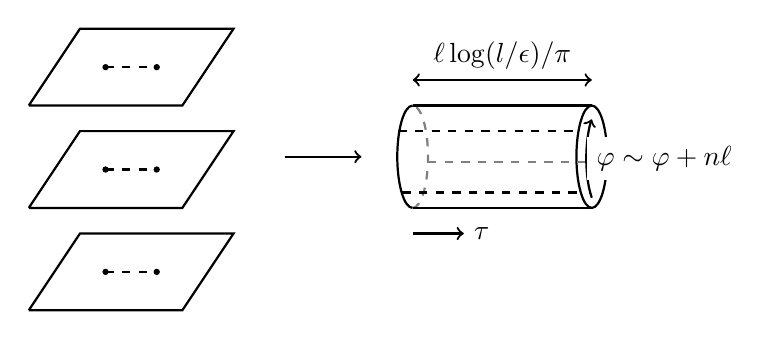
\begin{tikzpicture}[scale=0.65]
	\draw[thick] (2, 3) --++ (3, 0) --++ (1, 1.5) --++ (-3, 0) --++ (-1, -1.5);
	\draw[thick, dashed] (3.5, 3.75) --++(1,0);
	\filldraw [fill=black] (3.5, 3.75) circle (0.05);
	\filldraw [fill=black] (4.5, 3.75) circle (0.05);
	\draw[thick] (2, 1) --++ (3, 0) --++ (1, 1.5) --++ (-3, 0) --++ (-1, -1.5);
	\draw[thick, dashed] (3.5, 1.75) --++(1,0);
	\filldraw [fill=black] (3.5, 1.75) circle (0.05);
	\filldraw [fill=black] (4.5, 1.75) circle (0.05);
	\draw[thick] (2, -1) --++ (3, 0) --++ (1, 1.5) --++ (-3, 0) --++ (-1, -1.5);
	\draw[thick, dashed] (3.5, -0.25) --++(1,0);
	\filldraw [fill=black] (3.5, -0.25) circle (0.05);
	\filldraw [fill=black] (4.5, -0.25) circle (0.05);

	\draw[thick, ->] (7,2) --++ (1.5,0);

	\draw[thick] (9.5,1) arc (270:90:0.3 and 1);
	\draw[thick, dashed, color=gray] (9.5,1) arc (-90:90:0.3 and 1);
	\draw[thick] (13,2) ellipse (0.3 and 1);
	\draw[thick] (9.5,3) -- (13,3);
	\draw[thick] (9.5,1) -- (13,1);
	\draw[thick, dashed] (9.3, 1.3) --++ (3.5,0);
	\draw[thick, dashed] (9.22, 2.5) --++ (3.5,0);
	\draw[thick, dashed, color=gray] (9.8, 1.9) --++ (3.5,0);
	\draw[thick, ->] (9.5,0.5) --++ (1,0) node[right] {$\tau$};
	\draw[thick, ->] (13,1.2) arc (230:130:0.3 and 1) node[fill=white, right, midway] {$\varphi \sim \varphi + n\ell$};
	\draw[thick, <->] (9.5,3.5) -- node[above] {$\ell \log (l/\epsilon)/\pi$} (13,3.5);
\end{tikzpicture}
\caption{\label{fig:CFT2EE} The $n$-fold cover $\CM_n$ of $\BC$ with a cut between $z=-l/2$ and $l/2$ is conformally mapped to a cylinder.
The intervals are mapped to lines at $\varphi = k \ell$ $(k=0,1,\cdots, n-1)$ where the $n$ copies are glued together.
This shows the conformal transformation for $n=3$.
}
\end{figure}

The stress tensor in the holomorphic sector transforms under the conformal mapping as
\begin{align}\label{HolTra}
	T(z) = \left( \frac{\d w}{\d z}\right)^2 T(w) + \frac{c}{12}\{ w, z\} \ ,
\end{align}
where $\{ w, z\} \equiv w'''(z)/w'(z) - 3[ w''(z)/w'(z)]^2/2$ is the Schwarzian derivative, and similarly for the antiholomorphic sector.\footnote{We consider a theory only  with equal left and right central charges $c_L=c_R = c$. A theory with $c_L\neq c_R$ has a gravitational anomaly and the entanglement entropy of such a theory was studied by \textcite{Castro:2014tta,Azeyanagi:2015uoa,Nishioka:2015uka,Hughes:2015ora,Iqbal:2015vka}.}
We parametrize the cylinder of circumference $n\ell$ by the complex coordinate $w$ and map it to a complex plane parametrized by $z$ using the conformal transformation of Eq.\,\eqref{ConfMapCyl} with $\ell$ and $\zeta$ replaced with $n\ell$ and $z$, respectively.
Using Eq.\,\eqref{HolTra}, we find the Hamiltonian along the $\tau$ direction on the cylinder,
\begin{align}\label{CylHam}
\begin{aligned}
	H &= \int_0^{n\ell} \frac{\d\varphi}{2\pi} \left(T(w) + \bar T(\bar w)\right) \ , \\
		&= \frac{2\pi}{n\ell} \left( L_0 + \bar L_0 - \frac{c}{12} \right) \ ,
\end{aligned}
\end{align}
where $L_0\, (\bar L_0)$ is the Virasoro generator in the (anti-)holomorphic sector on $\BC$.
 
The ground state $|0\rangle$ is annihilated by $L_0$ and $\bar L_0$, hence the partition function Eq.\,\eqref{CylinderPF} with the Hamiltonian \eqref{CylHam} resulting in
\begin{align}
	\log Z[\CM_n] = \frac{c }{6n} \log \frac{l}{\epsilon} \ .
\end{align}
The entanglement entropy follows from Eq.\,\eqref{EE_PF},
\begin{align}
	S_A = \frac{c}{3}\log \frac{l}{\epsilon} \ ,
\end{align}
which agrees with the previous result Eq.\,\eqref{EE_CFT2} derived with the conformal anomaly.




\subsection{R{\'e}nyi entropy and conformal maps}\label{ss:Renyi_CFT}

In this section, we are concerned with the R{\'e}nyi entropy $S_n$, Eq.\,\eqref{Renyi_QFT}, for a spherical entangling surface in CFT and discuss the connection to a thermal entropy on a conformally flat space.

First, let $F_n \equiv - \log Z_n$ be a free energy for the partition function $Z_n$ on the $n$-fold cover, then the R{\'e}nyi entropy takes the following form:
\begin{align}\label{RenyiNewDef}
S_n = \frac{n F_1 - F_n}{1-n} \ .
\end{align}
Calculating the free energy $F_n$ on the $n$-fold cover is far from reach even in CFT, but if we restrict our attention to a spherical entangling surface in CFT, we are able to find universal results for the R{\'e}nyi entropy.

We locate a spherical entangling surface $\BS^{d-2}$ at $\rho=R$ (and $t=0$) in the Euclidean polar coordinates,
\begin{align}\label{CFT_Flat}
\d s^2_\text{Flat} = \d t^2 + \d\rho^2 + \rho^2 \d\Omega_{d-2}^2 \ .
\end{align}
The conformal symmetry allows one to connect various geometries that are  conformally equivalent to the metric Eq.\,\eqref{CFT_Flat}, which simplifies the calculation of $F_n$ as we will see below.


\subsubsection{Conformal map to hyperbolic coordinates}\label{ss:Rel_to_Therm}
We first map the flat space $\BR^d$ to a hyperbolic space $\BS^1 \times \BH^{d-1}$ with the metric
\begin{align}\label{CFT_Hyp}
\d s^2_\text{Hyp} = \d\tau^2 + \d u^2 + \sinh^2 u \,\d\Omega_{d-2}^2 
\end{align}
with the ranges $0\le \tau \le 2\pi$ and $0\le u <\infty$, by the coordinate transformation 
\begin{align}\label{BoundaryCM}
\begin{aligned}
t &= R \frac{ \sin\tau}{\cosh u + \cos\tau} \ , \qquad
\rho = R \frac{\sinh u}{\cosh u + \cos\tau} \ .
\end{aligned}
\end{align}
The two metrics are conformally equivalent:
\begin{align}
	\d s^2_\text{Flat} = \Omega^2_\text{Hyp}\, \d s^2_\text{Hyp} \ ,	
\end{align}
with the conformal factor
\begin{align}
	\Omega_\text{Hyp} = \frac{R}{\cosh u + \cos \tau} \ .
\end{align}
Under this coordinate transformation, the entangling surface at $\rho=R$ is mapped to a sphere $\BS^{d-2}$ at $u=\infty$ in the hyperbolic coordinates.
The $n$-fold cover $\CM_n$ around the entangling surface at $\rho= R$ in Eq.\,\eqref{CFT_Flat} is equivalent to extending the ranges of $\tau$ to $0\le \tau \le 2\pi n$ (see Fig.\,\ref{fig:ConformalMap}).
After this conformal map, CFT is defined on the hyperbolic space $\BH^{d-1}$ at temperature $T_n=1/(2\pi n)$.


\begin{figure*}[htbp]
\centering
\begin{tikzpicture}[scale = 1.3, baseline={([yshift=-.5ex]current bounding box.center)}, scale=0.7]
\draw [->, thick] (-0.5,0) -- (-0.5,3) node [above] {$t$};
\draw [thick] (0,0.5) --++ (3,0) --++ (1,2) --++ (-3,0) -- (0,0.5);
\draw [thick, orange] (1.14,1.65) arc [start angle = 150, end angle = 280, radius = 0.3];
\draw [thick, dashed, tsuyukusairo, fill=white] (2,1.5) circle [x radius = 0.7, y radius = 0.4, rotate = 360];
\node [fill=white]  at (3.1, 1){$\BS^{d-2}$};
\draw [thick, ->] (2,1.5) --++ (45:0.8) node [right] {$\rho$};
\draw [thick, orange, fill=white] (1.7,1.5) arc [start angle = 0, end angle = 150, radius = 0.3];
\draw [thick, <-, orange] (1.7,1.5) arc [start angle = 360, end angle = 310, radius = 0.3];
\node at (2,-1) {$\BR^{d}$};
\node at (2,-2) {\footnotesize $\d s_\text{Flat}^2 = \d t^2 + \d\rho^2 + \rho^2 \,\d\Omega_{d-2}^2$};
\end{tikzpicture}
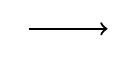
\begin{tikzpicture}[baseline={([yshift=-.ex]current bounding box.center)}, scale=0.5]
\draw[thick, ->] (1, 0) --++(2,0);
\end{tikzpicture}
%
\begin{tikzpicture}[scale=1.2, baseline={([yshift=1.2ex]current bounding box.center)}, scale=0.7]
\draw[thick] (0,3) arc [start angle = 90, end angle = 270, x radius = 0.2, y radius = 0.5];
\draw[thick, dashed] (0,2) arc [start angle = 270, end angle = 450, x radius = 0.2, y radius = 0.5];
\draw [thick] (4,2.5) circle [x radius = 0.2, y radius = 0.5, rotate = 0];
\node at (4.6,2.5) {$\tau$};
\draw [thick] (0,3) -- (4,3);
\draw [thick] (0,2) -- (4,2);
\draw[thick] (0,1.6) arc [start angle = 90, end angle = 270, x radius = 0.2, y radius = 0.8];
\draw[thick, dashed] (0,0) arc [start angle = 270, end angle = 450, x radius = 0.1, y radius = 0.8];
\draw[thick, orange,
	decoration={markings, mark=at position 0.5 with {\arrow{<}}},
        postaction={decorate}] (2,3) arc [start angle = 90, end angle = 270, x radius = 0.2, y radius = 0.5];
\draw[thick, dashed, orange] (2,2) arc [start angle = 270, end angle = 450, x radius = 0.1, y radius = 0.5];
\draw [thick, tsuyukusairo] (4,0.8) circle [x radius = 0.1, y radius = 0.8, rotate = 0];
\draw [thick] (0.05,1.55) arc [start angle = 190, end angle = 345, x radius = 2, y radius = 0.92];
\draw [thick] (3.94,0.1) arc [start angle = 15, end angle = 170, x radius = 2, y radius = 0.92];
\node at (4.9,0.8) {$\BS^{d-2}$};
\draw [->, thick] (2,-0.5) -- (4,-0.5) node [right] {$u$};
\node at (2,-1.5) {$\BS^{1} \times \BH^{d-1}$};
\node at (2,-2.5) {\footnotesize $\d s^2_\text{Hyp} = \d\tau^2 + \d u^2 + \sinh^2 u\, \d\Omega_{d-2}^2$};
\end{tikzpicture}
%
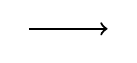
\begin{tikzpicture}[baseline={([yshift=-.5ex]current bounding box.center)}, scale=0.5]
\draw[thick, ->] (1, 0) --++(2,0);
\end{tikzpicture}
\begin{tikzpicture}[scale=1.2, baseline={([yshift=3ex]current bounding box.center)}, scale=0.7]
\draw [thick] (0,0) -- (3,0);
\draw [thick, tsuyukusairo] (0,1) circle [x radius = 0.3, y radius = 0.5, rotate = 360];
\node at (-0.9,1) {$\BS^{d-2}$};
\draw [thick] (0,1.5) -- (3,1) -- (0, 0.5);
\draw [thick, orange,
	decoration={markings, mark=at position 0.5 with {\arrow{<}}},
        postaction={decorate}] (3,2) circle [x radius = 0.3, y radius = 0.5, rotate = 360];
\node at (3.6,2) {$\tau$};
\draw [thick] (3, 2.5) -- (0,2) -- (3, 1.5);
\filldraw [fill=black] (0,0) circle (0.1) node [below] {$\theta=0$};
\filldraw [fill=black] (3,0) circle (0.1) node [below] {$\pi/2$};
\node at (1.5,-1.5) {$\BS^{d}$};
\node at (1.5,-2.5) {\footnotesize $\d s^2_\text{Sp} = \d\theta^2 + \sin^2\theta\, \d\tau^2 + \cos^2\theta\, \d\Omega_{d-2}^2$};
\end{tikzpicture}
\caption{\label{fig:ConformalMap}  The coordinate transformation Eq.\,\eqref{BoundaryCM} induces the conformal map from a flat space [Left] to a hyperbolic space times a circle [Middle].
The latter is further conformally mapped to a sphere [Right] by the coordinate transformation, $\sinh u = \cot\theta$.
The blue circles represent the entangling surface $\BS^{d-2}$, and the orange circles with arrows stand for the modular time, respectively.
}
\end{figure*}

We assume there are no conformal anomalies (i.e., $d$ is odd) for the moment. Then the partition function is invariant under the conformal map; hence on the hyperbolic coordinates Eq.\,\eqref{CFT_Hyp}, $Z_n$ is the thermal partition function
\begin{align}\label{PFHyp}
Z_n = \tr \left(e^{-H_\text{Hyp} /T_n}\right) \ ,
\end{align}
where $H_\text{Hyp}$ is the Hamiltonian generating the translation along $\tau$ on $\BH^{d-1},$\footnote{The Hamiltonian or the energy is given by the generator of $\tau$ translation $T_{\mu\nu}\xi^\mu$ with $\xi^\mu\partial_\mu = \partial_\tau$ integrated over a spacelike surface
\begin{align}
H  =\int_{\BH^{d-1}}\d^{d-1}x\, \sqrt{g} \, T_{\mu\nu}(x)\,\xi^\mu n^\nu \ ,
\end{align}
where $n^\mu\partial_\mu = \sqrt{g^{\tau\tau}} \partial_\tau$ is the unit normal vector.
}
\begin{align}\label{ModularHamiltonian}
H_\text{Hyp}  =  \int_{\BH^{d-1}}\d^{d-1}x\, \sqrt{g} \, T_{\tau\tau}(x) \ .
\end{align}
The free energy $F_n = -\log Z_n$ and the thermal free energy $F(T)$ on $\BH^{d-1}$ at temperature $T=T_n$ are related by $F_n = F(T_n)/T_n$. 
Using the thermodynamic identity $S_\text{therm}(T) = - \partial F(T)/\partial T$, the R{\'e}nyi entropy Eq.\,\eqref{RenyiNewDef} is given by the integral of the thermal entropy \cite{Hung:2011nu},
\begin{align}\label{RenyiTherm}
\begin{aligned}
S_n &= \frac{n}{1-n} \frac{F(T_1) - F(T_n)}{T_1} \ , \\
	&= \frac{n}{n-1}\frac{1}{T_1} \int_{T_n}^{T_1} \d T \, S_\text{therm}(T) \ .
\end{aligned}
\end{align}
This is an intriguing connection between the R{\'e}nyi entropy of a spherical entangling surface on the flat space and the thermal entropy on $\BH^{d-1}$ at finite temperature, which will be useful for the holographic studies in the following sections.
Moreover, it follows from the $n\to 1$ limit of Eq.\,\eqref{RenyiTherm} that the entanglement entropy equals the thermal entropy at temperature $T= T_1$,
\begin{align}\label{RenyiAndTherm}
S_1 = \lim_{n\to 1} S_n = S_\text{therm}(T_1) \ .
\end{align}
There is a subtle issue in this relation associated with the boundary of the hyperbolic space in even dimension \cite{Casini:2011kv}.
The universal logarithmic divergence proportional to the type $A$ anomaly in the entanglement entropy \eqref{EE_Even} is attributed to a boundary effect \cite{Herzog:2015ioa,Herzog:2016kno}.




\subsubsection{Conformal map to spherical coordinates}
We can make a further conformal transformation from the hyperbolic coordinates
 Eq.\,\eqref{CFT_Hyp} to the spherical coordinates $\BS^{d}$ of unit radius,
\begin{align}\label{CFT_Sphere}
\d s^2_\text{Sp} = \d\theta^2 + \sin^2 \theta\, \d\tau^2 + \cos^2\theta\, \d\Omega_{d-2}^2 \ ,
\end{align}
with the ranges $0\le \tau \le 2\pi$ and $0\le \theta \le \pi/2$,
by the coordinate transformation $\sinh u = \cot\theta$ (see Fig.\,\ref{fig:ConformalMap}).
It is also conformally equivalent to the flat space
\begin{align}
	 \d s^2_\text{Flat} = \Omega^2_\text{Sp}\,\d s^2_\text{Sp}
\end{align}
with the conformal factor
\begin{align}
	\Omega_\text{Sp}= \frac{R}{1 + \sin\theta\, \cos\tau} \ .
\end{align}

The $n$-fold cover $\CM_n$ of $\BR^d$ is conformally equivalent to the $n$-fold cover of the $d$-sphere $\BS_n^d$ with the extended range $0\le \tau \le 2\pi n$, and 
the free energy $F_n$ equals to the logarithm of the partition function $Z[\BS^d_n]$ for CFT,
\begin{align}\label{F_nZ}
F_n = -\log Z[\BS^d_n] \ .
\end{align}
The R{\'e}nyi entropies for free fields were computed by \textcite{Klebanov:2011uf}
based on  Eq.\,\eqref{F_nZ} and shown to agree with the calculation on the hyperbolic coordinates.


Next we look into Eq.\,\eqref{RenyiAndTherm}, the entanglement entropy to the thermal entropy.
Through the thermodynamic relation, $S_\text{therm}$ is given by the free and total energies $F(T), E(T)$ of the CFT$_d$,
\begin{align}\label{TDR_CFT}
S_\text{therm}(T) = \frac{E(T) - F(T)}{T} \ .
\end{align}
When $d$ is odd, the total energy vanishes for CFT$_d$ because the round sphere $\BS^d$ is conformally equivalent to the flat space $\BR^d$: $E(T)=0$ \cite{Casini:2011kv,Klebanov:2011uf}.
Combining Eqs.\,\eqref{RenyiAndTherm} and \eqref{TDR_CFT} with $F(T_1)/T_1 = F_1 = -\log Z[\BS^d_n]$, we obtain the equality between the entanglement entropy of a sphere $\BS^{d-2}$ and the partition function on $\BS^d$,
\begin{align}\label{EE_F}
S_1 = \log Z[\BS^d] \ .
\end{align}
Note that this equality should be taken up to UV divergences as the vanishing of the total energy holds for CFT$_d$ only after renormalizing the divergences.
If the right-hand side is the correctly renormalized effective action, it should be identified with the universal part of the entanglement entropy in Eq.\,\eqref{EE_Odd}, 
\begin{align}
F = (-1)^{(d-1)/2}\log Z[\BS^d] \ .
\end{align}
This will be the key relation in Sec. \ref{ss:RGflow} when we construct a monotonically decreasing function along RG flows in odd dimensions.

When $d$ is even, there are conformal anomalies in the partition function $Z[\BS^d]$, which gives rise to the logarithmic divergence in entanglement entropy as appeared in Eq.\,\eqref{EE_Even}.
This is most easily seen by analytically continuing Eq.\,\eqref{EE_F} from odd to even dimensions and replacing the pole with the logarithm.


\subsection{Universal behavior of R{\' e}nyi entropy in CFT}
Having established the universal relation \eqref{EE_F} for the spherical entanglement entropy, we now seek for the universal aspects of the R{\'e}nyi entropies.
We set $R=1$ since the result should not depend on $R$ because of the conformal symmetry.

We want to examine the universal part of the spherical R{\'e}nyi entropy in odd dimensions and expand it around $n=1$ where $S_1 = -F_1$ up to the UV divergences. 
From Eq.\,\eqref{RenyiNewDef} we have the expansion
\begin{align}
\begin{aligned}
S_n &= S_1 + \frac{F_n - F_1}{n-1} \ , \\
	&= S_1 + \sum_{k=1}^\infty \frac{1}{k!} \frac{\partial^k F_n}{\partial n^k}\bigg|_{n=1} (n-1)^{k-1} \ .
\end{aligned}
\end{align}
For a spherical entangling surface in CFT, the free energy is given by the partition function \eqref{PFHyp} on the hyperbolic coordinates, which fixes the derivatives of $F_n$, 
\begin{align}
\begin{aligned}
\frac{\partial^k F_n}{\partial n^k}\bigg|_{n=1} &= - (-2\pi)^k \langle H_\text{Hyp}^k\rangle  \ , 
\end{aligned}
\end{align}
where $\langle\, \cdot\, \rangle \equiv \tr (\,\cdot\, e^{-2\pi H_\text{Hyp}})/\tr (e^{-2\pi H_\text{Hyp}})$ stands for the expectation value of an operator and we used the fact that the energy vanishes for CFT in odd dimensions: $E(T) = \langle H_\text{Hyp} \rangle= 0$.
The form of the Hamiltonian \eqref{ModularHamiltonian} on the hyperbolic space allows us to obtain the expansion in terms of the correlation functions of the stress tensors,
\begin{align}\label{REexpand}
\begin{aligned}
S_n &= S_1 \\
	&~- \sum_{k=1}^\infty \frac{(-2\pi)^{k+1}}{(k+1)!} (n-1)^k \\
	&\quad \cdot \int_{\BH^{d-1}}\!\cdots \int_{\BH^{d-1}}\prod_{i=1}^{k+1} \d^{d-1}x_i\,\sqrt{g}\, \langle T_{\tau\tau}(x_1) \cdots T_{\tau\tau}(x_{k+1}) \rangle \ .
\end{aligned}
\end{align}

The leading term is fixed by the two-point function of the stress tensors, whose integral results in \cite{Perlmutter:2013gua}
\begin{align}\label{LeadingRE}
\partial_n S_n\big|_{n=1} = -C_T\,\text{Vol}\left(\BH^{d-1}\right)\,\frac{\pi^{d/2+1}(d-1)\Gamma\left(d/2\right)}{\Gamma(d+2)} \ ,
\end{align}
where $C_T$ is a constant present in Eq.\,\eqref{TTCor}.
For odd $d$, the regularized volume of $\BH^{d-1}$ is [see \textcite{Klebanov:2011uf} for $d=3$]
\begin{align}\label{HypVolume}
\text{Vol}(\BH^{d-1}) = (-1)^{(d-1)/2}\frac{\pi^{d/2}}{\Gamma \left(d/2\right)} = \pi^{d/2-1}\Gamma(1-d/2)\ ,
\end{align}
which may be obtained by putting the cutoff $\Lambda\gg 1$ at the spatial infinity of $\BH^{d-1}$ and picking up a constant term in $\Lambda \to \infty$ limit.\footnote{In the second equality, we used the reflection formula for the gamma functions, $\Gamma(z) \Gamma(1-z) = \pi/ \sin (\pi z)= \pi (-1)^{(d-1)/2}$.}


While the universal result Eq.\,\eqref{LeadingRE} was derived under the assumption that $d$ is \emph{odd}, it is shown to hold for \emph{even} $d$ \cite{Perlmutter:2013gua} where there are additional terms including the one-point function $\langle\CH\rangle$ which no longer vanishes due to the conformal anomaly.
In addition, the volume of the hyperbolic space $\text{Vol}(\BH^{d-1})$ logarithmically diverges for even $d$ after regularizing the power law divergence, which may be inferred from Eq.\,\eqref{HypVolume} as a pole of the gamma function by analytically continuing odd $d$ to even.

We finally note that the first derivative of the sphere entanglement entropy Eq.\,\eqref{LeadingRE} can be useful to read off the coefficient $C_T$ of the two-point function of the stress tensor.
A similar expansion and a universal leading coefficient will be derived for a supersymmetric generalization of the R{\'e}nyi entropy in Sec. \ref{ss:SRE}.

\endinput